\documentclass{scrreprt}

\usepackage{aligned-overset}
\usepackage{amsmath}
\usepackage{amssymb}
\usepackage{bm}
\usepackage{chngcntr}
\usepackage[shortlabels]{enumitem}
\usepackage{hyperref}
\usepackage[utf8]{inputenc}
\usepackage{mathtools}
\usepackage{physics}
\usepackage{tabularx}
\usepackage{titling}
\usepackage{fancyhdr}
\usepackage{xfrac}
\usepackage[table]{xcolor}
\usepackage{pgfplots}

%% Fix equation numbering for scrreprt class.
\counterwithout{equation}{chapter}

\pgfplotsset{compat = newest}
\usepgfplotslibrary{patchplots}
\usetikzlibrary{intersections}
\usetikzlibrary{shapes}
\usetikzlibrary{patterns}
\usepgfplotslibrary{fillbetween}

\author{Karsten Lehmann}
\date{SoSe 2021}
\title{Übung 12 Analysis - Weiterführende Konzepte}

\pagestyle{fancy}
\fancyhf{}
\lhead{\thetitle}
\rhead{\theauthor}
\lfoot{\thedate}
\rfoot{Seite \thepage}

\newcommand\skalprod[1]{\left\langle #1 \right\rangle}
\newcommand\nnorm[1]{\left\lvert\left\lvert\left\lvert #1 \right\rvert\right\rvert\right\rvert}

\begin{document}
\setcounter{chapter}{1}
\section*{Extremalaufgaben mit Gleichungsnebenbedingungen}

\paragraph{Aufgabe 1} Ermitteln Sie mit Hilfe der Methode der
Lagrange-Multiplikation diejenigen Punkte $Q = (x, y)$ auf der Hyperbel
$M = \qty{(x, y) \in \mathbb{R}^2 \colon y^2 - x^2 = 1}$, die vom Punkt
$P = (1, 0)$ den kürzesten Abstand haben.
Berechnen Sie den Abstand $d(P, Q)$ von $P$ und $Q$.
Überlegen Sie sich, warum für der ermittelten Punkte tatsächlich der
kürzeste Abstand ermittelt wurde.

\subparagraph{Lösung:} $M = \qty{(x, y) \in \mathbb{R}^2 \colon y^2 - x^2 = 1}$
ist nicht offen.
\begin{center}
  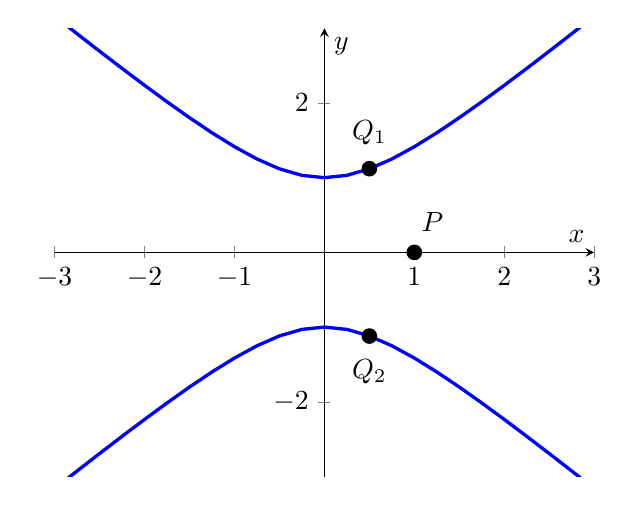
\begin{tikzpicture}
    \begin{axis}[
        axis lines=middle,
        xlabel=$x$,
        xmax = 3,
        xmin = -3,
        ylabel=$y$,
        ymax = 3,
        ymin = -3,
      ]
      \addplot[
        domain = -3:3,
        very thick,
        blue,
      ] {sqrt(x^2 + 1)};
      \addplot[
        domain = -3:3,
        very thick,
        blue,
      ] {-1 * sqrt(x^2 + 1)};
      \node[circle, fill, inner sep=2pt] at (0.5,1.12){};
      \node[circle, fill, inner sep=2pt] at (1,0){};
      \node[circle, fill, inner sep=2pt] at (0.5,-1.12){};
      \node at (1.2, 0.4) {$P$};
      \node at (0.5, 1.6) {$Q_1$};
      \node at (0.5, -1.6) {$Q_2$};
    \end{axis}
  \end{tikzpicture}
\end{center}
$h(x, y) = y^2 - x^2 - 1$ ist stetig differenzierbar.
$M = h^{-1} ({0})$. Aus \textbf{Proposition 6.3.3}
\textit{``Stetige Urbilder abgeschlossener Mengen sind abgeschlossen''} folgt
$M$ ist abgeschlossen.

\textbf{Existieren Extremalstellen von stetigen Funktionen auf $M$?}
\[
  d(\underset{(x, y)}{\underbrace{Q}}, \underset{(1, 0)}{\underbrace{P}})
  = \norm{\overrightarrow{PQ}}_2
  = \qty\Big(\qty(x - 1)^2 + y^2)^{\frac{1}{2}}
\]
\[
  f(x, y) = d(Q, P)^2 = (x - 1)^2 + y^2
\]
$d(\cdot, P)$ und $f$ haben gleiches Monotonieverhalten für $d(\cdot, P) \geq 0$.

\textbf{Problem:} $f(x, y) \longrightarrow \min$ bei $(x, y) \in M$.

Lagrange-Funktion: $F(x, y, \lambda) = f(x, y) + \lambda \cdot h(x, y)$
\begin{itemize}
\item $f, h$ sind stetig differenzierbar mit $\nabla f(x, y) = \begin{pmatrix}
    2 \qty\big(x - 1) \\
    2 y
  \end{pmatrix}$ und $\nabla h(x, y) = \begin{pmatrix}
    -2 x \\
    2 y
  \end{pmatrix}$
\item Regularitäts- / Rangbedingung: Jacobi-Matrix der Nebenbedingung besitzt Vollrang.
  \[
    J_h(x, y) = \nabla h(x, y)^T \ne \begin{pmatrix}0 & 0\end{pmatrix}
  \]
  Es gilt $\nabla h(x, y) = \begin{pmatrix}-2x \\ 2y \end{pmatrix} =
  \begin{pmatrix}0 \\ 0\end{pmatrix} \iff x = y = 0$, aber $(0, 0) \notin M$

  $\Rightarrow$ Rangbedingung gilt.
\end{itemize}

Falls $\qty(\overline{x}, \overline{y})$ eine lokale Extremalstelle von $f$ auf
$M$ ist, so existiert ein $\overline{\lambda} \in \mathbb{R}$, so dass
$\qty(\overline{x}, \overline{y}, \overline{\lambda}) \in M \times \mathbb{R}$
eine freie lokale Extremalstelle von $F$ ist.

$F \colon \mathbb{R}^3 \to \mathbb{R}$ ist stetig differenzierbar.
Notwendige Qptimalitätsbedingung:
$\nabla F(\overline{x}, \overline{y}, \overline{\lambda}) = (0, 0, 0)$.
\setcounter{section}{1}
\begin{align}
  \frac{\partial F}{\partial x} (\ldots) &= 2(x - 1) - 2 \lambda x
  = 2(x(1 - \lambda) - 1) = 0 & \label{eq:1} \\
  \frac{\partial F}{\partial y} (\ldots) &= 2y + 2\lambda y = 2y(1 + \lambda) = 0 \label{eq:2} \\
  \frac{\partial F}{\partial \lambda} (\ldots) &= h(x, y) = y^2 - x^2 - 1 = 0 \label{eq:3}
\end{align}
$\Rightarrow$ nichtlineares Gleichungssystem.

$\hyperref[eq:2]{(2)} \iff y = 0 \lor \lambda = -1$

$y = 0$ in $\hyperref[eq:3]{(3)}$ einsetzen führt zu $-x^2 - 1 = 0$, nicht lösbar.
$\Rightarrow y \ne 0 \land \lambda = -1$

$\lambda = -1$ in $(1)$ einsetzen: $2x - 1 = 0 \Rightarrow x_1 = \frac{1}{2}$

$x_1 = \frac{1}{2}$ in $\hyperref[eq:3]{(3)}$ einsetzen:
$y^2 = \frac{5}{4}, y_{1|2} = \pm \frac{\sqrt{5}}{2}$.

Kritische Punkte: $\qty(x_1, y_1) = \qty(\frac{1}{2}, \frac{\sqrt{5}}{2})$,
$\qty(x_2, y_2) = \qty(\frac{1}{2}, - \frac{\sqrt{5}}{2})$ mit
$f\qty(x_k, y_k) = \frac{3}{2}$ und $d\qty(Q_k, P) = \sqrt{\frac{3}{2}}$.

Wir betrachten
$M_0 \coloneqq M \cap \qty{(x,y) \in \mathbb{R}^2 {\Big |}
  f(x, y) \leq f\qty(x_k, y_k) = \frac{3}{2}}
= h^{-1}(\qty{0}) \cap f^{-1}\left( \left(-\infty, \frac{3}{2}\right] \right)$

$\Rightarrow M_0$ ist abgeschlossen, da $h, f$ stetig und
${0}, {-\infty, \frac{3}{2}}$ abgeschlossen sind.

Angenommen $M_0$ ist nicht beschränkt, dann existiert eine Folge
$\qty(x_n, y_n)_{n \in \mathbb{N}}$ in $M_0$ mit
$\norm{\qty(x_n, y_n)}_2 \overset{n \to \infty}{\longrightarrow} +\infty$,
Widerspruch zu
$\qty(x_n, y_n) \in f^{-1}\left(\left(-\infty, \frac{3}{2}\right]\right)$.

$\Rightarrow M_0$ ist beschränkt und somit kompakt. Nach Weierstraß besitzt
$f$ auf $M_0$ globale Minimalstellen, die auch globale Minimalstellen von
$f$ auf $M$ sind.

$\Rightarrow f$ besitzt lokale Minimalstellen auf $M$

$\Rightarrow$ Diese befinden sich unter den kritischen Punkten.

Wegen $f\qty(x_k, y_x) = \frac{3}{2}$ sind $\qty(x_1, y_1), \qty(x_2, y_2)$
die globalen Minimalstellen.

\end{document}